% !TeX root = bericht.tex
\section{Aufgabe 2 - Regelung mit einem P-Regler}
Das Ziel dieser Aufgabe ist es, die Drehzahl des Gleichstrommotors mit einem P-Regler zu regeln.
\subsection{Signalflussbild}
Wir verwenden die Regelstrecke aus Kapitel \ref{subsec:signalflussbild} und fügen davor einen P-Regler hinzu.
Zwischen Regler und Regelstrecke wird noch ein Saturation-Block hinzugefügt, um die maximale Spannung von $\pm \SI{10}{\volt}$ zu begrenzen.
\begin{figure}[H]
    \centering
    
\includegraphics[width=0.9\textwidth]{p-regler_sim.png}
    \caption{Signalflussbild der Regelung mit einem P-Regler}
\end{figure}

\subsection{Regelung auf \SI{100}{\radian\per\second}}
\label{sub:p_regler}
Das Ziel ist es, die Drehzahl auf \SI{100}{\radian\per\second} zu regeln.
Dazu müssen wir den Verstärkungsfaktor $K_r$ des P-Reglers so wählen, sodass der Motorsteuerung gerade nicht in die Begrenzung geht.
Wir können eine maximale Regeldifferenz von $\pm \SI{100}{\radian\per\second}$ erhalten (z.B. wenn wir den Motor von \SI{0}{\radian\per\second} auf \SI{100}{\radian\per\second} beschleunigen wollen).
Die Stellgröße kann maximal $\pm \SI{10}{\volt}$ betragen, da dies die maximale Spannung ist, die der Motor akzeptieren kann.
Daher muss der Verstärkungsfaktor $K_r$ so gewählt werden, dass
$$\SI{100}{\radian\per\second} \cdot K_r = \SI{10}{\volt}$$
gilt.
Daraus ergibt sich, dass $K_r = 0.1$ sein muss, um die Drehzahl auf \SI{100}{\radian\per\second} zu regeln.
\begin{figure}[H]
    \centering
    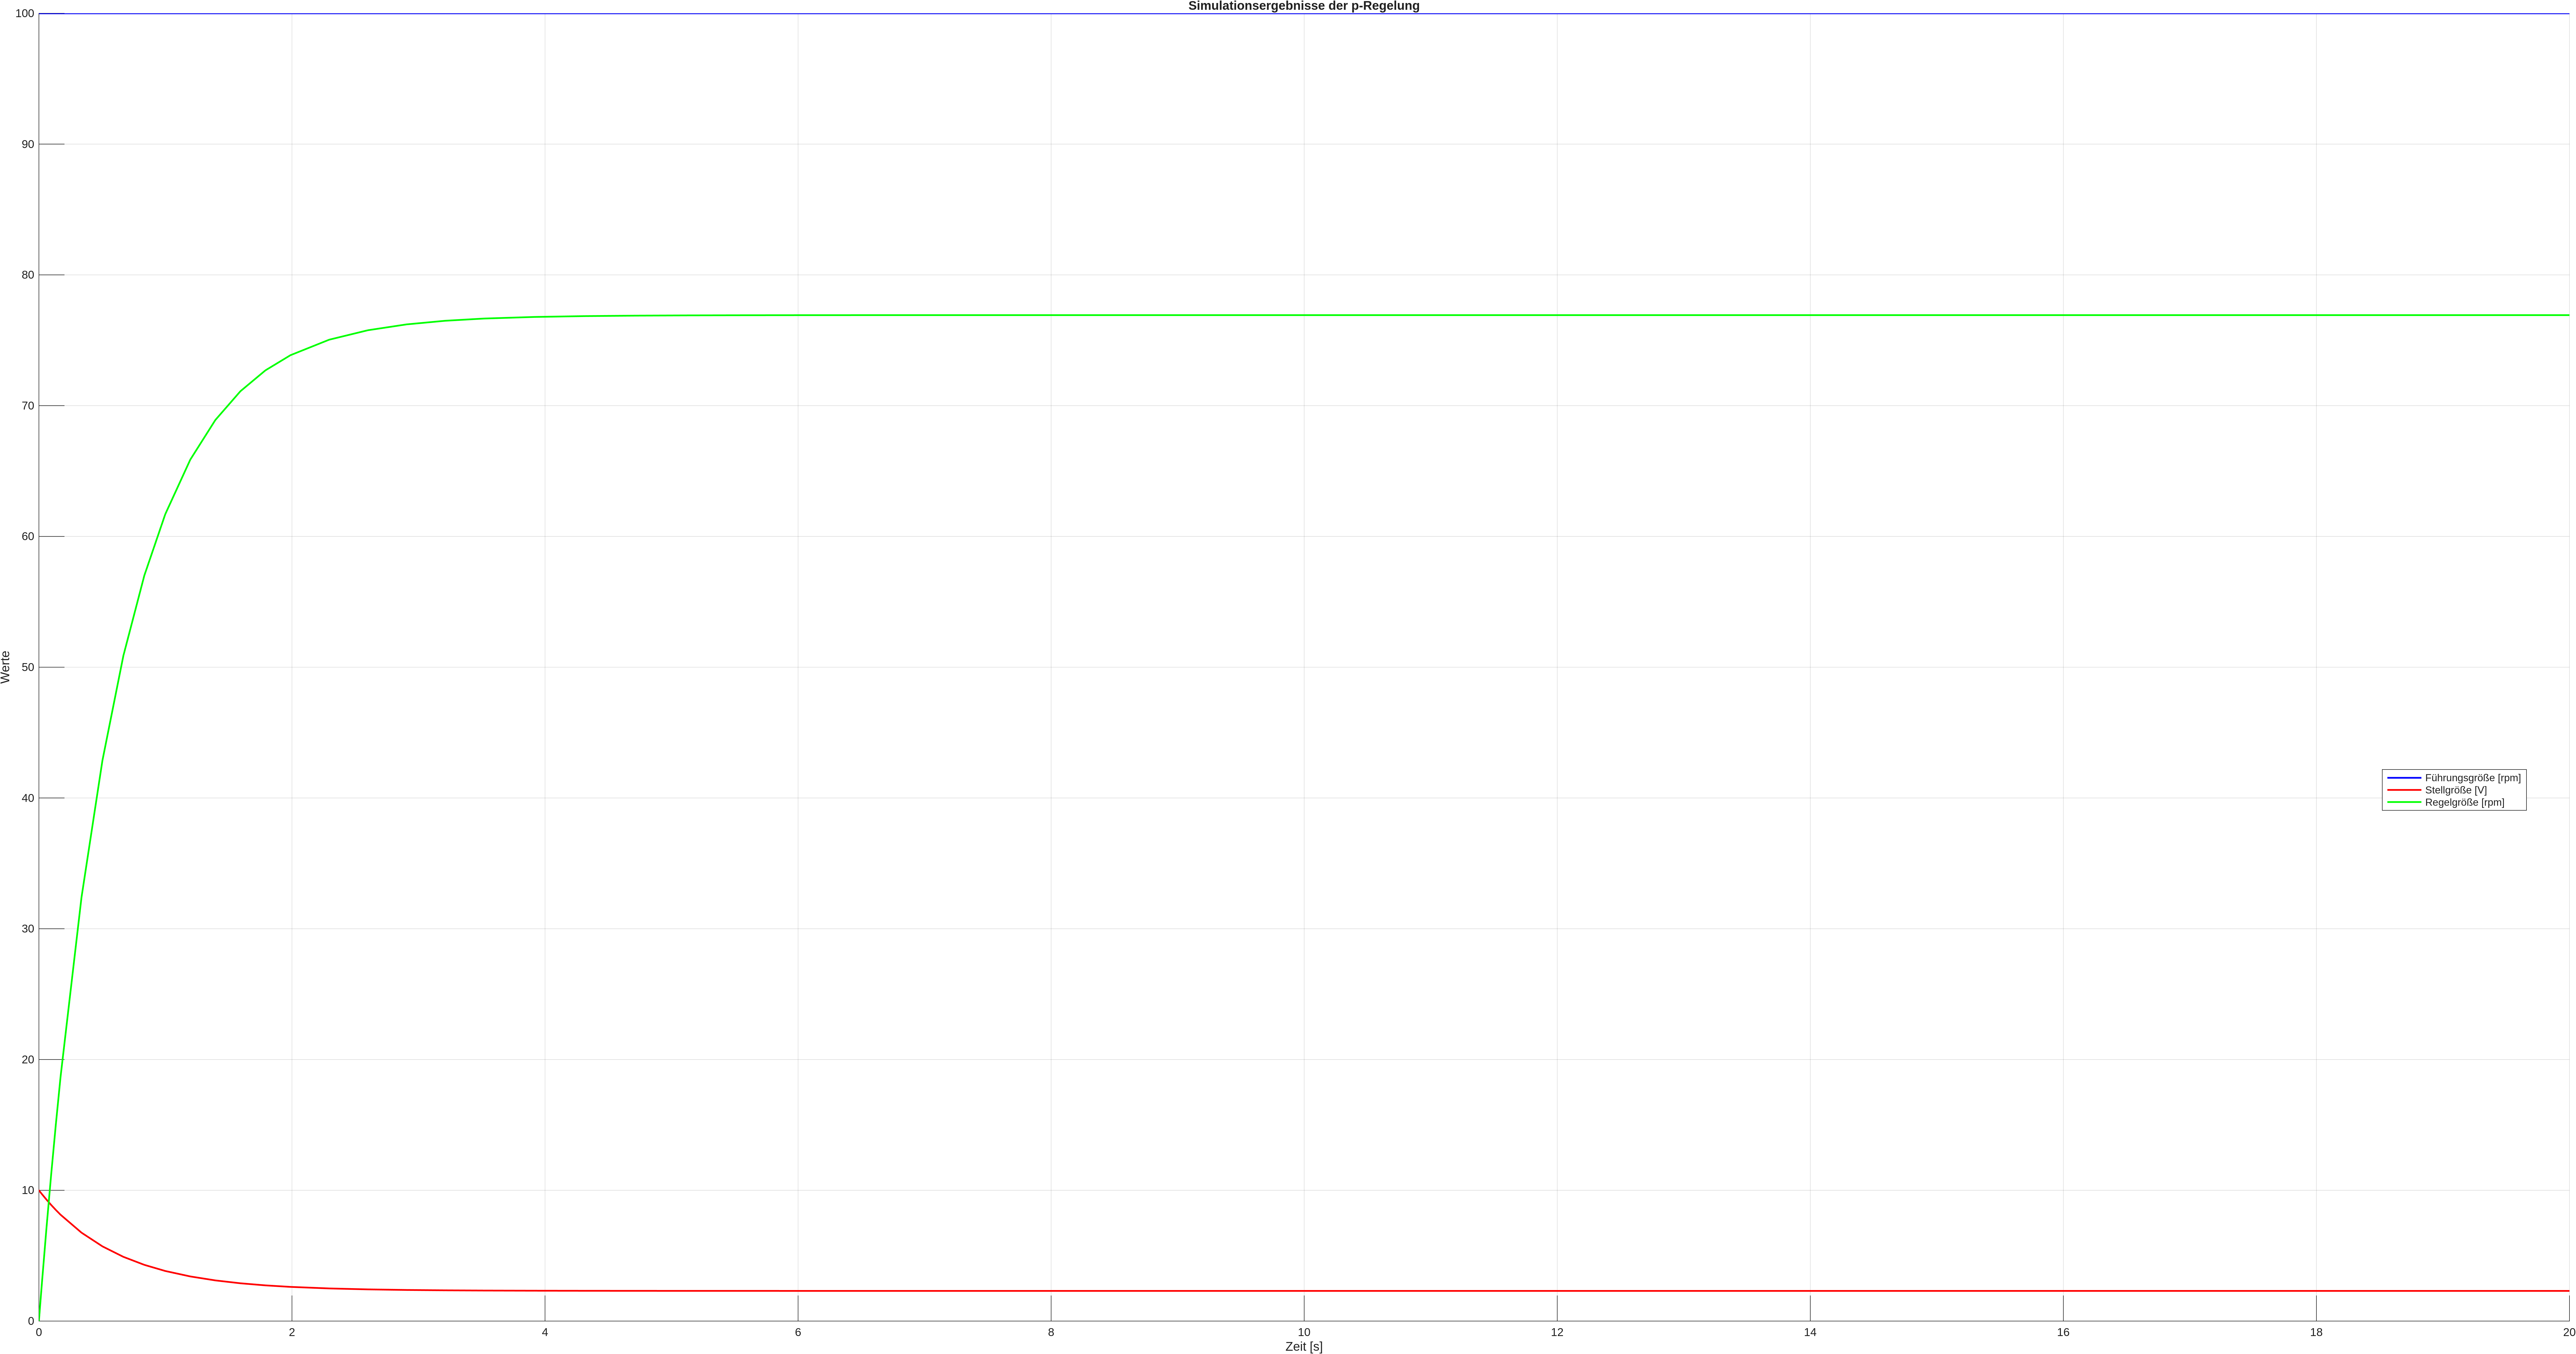
\includegraphics[width=0.9\textwidth]{images/a2_p_regelung_sim.png}
    \caption{Simulationsergebnis der Regelung mit einem P-Regler auf \SI{100}{\radian\per\second}}
    \label{abb:p_regler}
\end{figure}
Man erkennt, dass die Drehzahl nicht die gewünschte Führungsgröße von \SI{100}{\radian\per\second} erreichen kann. 
Daher ist der P-Regler hier stationär ungenau. 